This section details the controller design process for the bicycle, where three controller types were investigated: \textit{PID}, \textit{LQR}, and \textit{$H_{\infty}$ loop-shaping}. Since the steering angle is the only control variable and the lean angle is the only measured variable, the controller design problem is a \textit{single-input, single-output} (SISO) type. \\

For simulation, the second order non-linear model derived in the previous section will be used to test the suitability of the final controller designs. This is to determine if the controller will still manage to stabilise the bicycle, even if it is perturbed outside of the linear range the controller is designed for. Thus, all following plots are using the non-linear model. \\

The simulation and development environment was chosen to be Matlab and Simulink. Additionally, a bicycle simulator was developed from first principles using the game engine \textit{Unity} and C\#. This gives a full 3D representation of the bicycle dynamics and allows real-time simulation, where the user can impose disturbances, and change various parameters on the fly, such as controller gains, sensor noise, actuator limits, and so forth. The  non-linear differential equation of the second order model was integrated using the fourth order \textit{Runge-Kutta} method. A screenshot of the custom simulator is given in Figure \ref{fig:bikesim} below.

\begin{figure}[H]
	\centering
	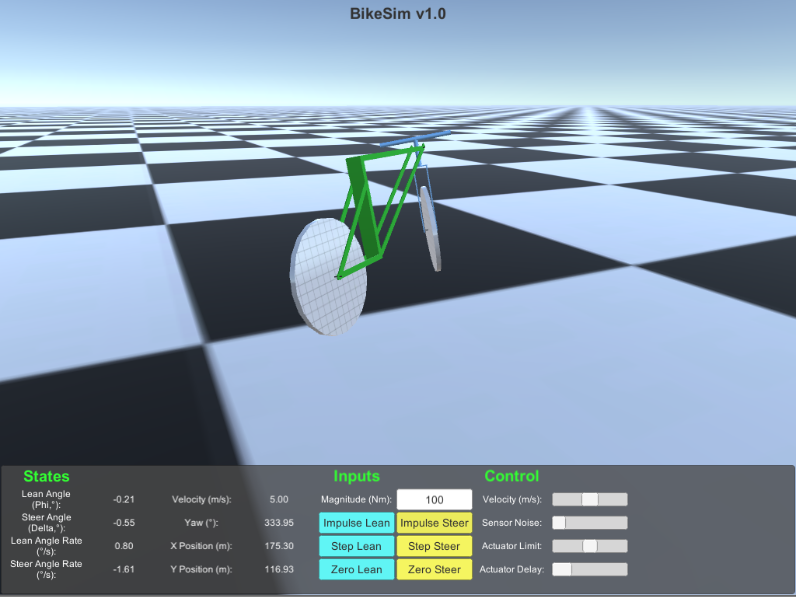
\includegraphics[scale=0.6]{BikeSim}
	\caption{Custom Bicycle Simulator}
	\label{fig:bikesim}
\end{figure}

For the sake of brevity, this section will only give detailed explanations of the controller design process for \textit{one} of the two bicycles, namely the Lego prototype. The controller designs for the full-scale bicycle follow essentially the same logic, given that the plant and actuator models are of the same form, and thus the design steps need only be described once. However, the final controller designs and their performance in simulation will be given for both bicycles.

\subsection{Performance Requirements}
When designing a control system, it is important to be aware of any requirements and specifications that need to be met as to tailor the control law to those needs. In the case of the rider-less bicycle, the main goal is to ensure stability across a relatively broad range of forward speeds.\\

In addition, should stability be achieved, it is desirable to have a controller that is primarily focused on reducing the effects of disturbances acting on the bicycle, as opposed to tracking the reference since this will be predominantly set to zero. Disturbances could be as small as an uneven road or path that the bicycle is riding over, and as large as a strong gust of wind giving the bicycle a sideways push. As a further consideration, the amount of overshoot should be limited, so as not to excite any non-linearities by deviating too far from the linear operating point the controller is designed for. \\

For all controllers, the output is limited to $\pm 60$ degrees to prevent extreme steering angles. \\

Furthermore, the cross-over frequency needs to be kept above the frequency of the right-half plane pole, as there the phase lead provided by the pole is needed to ensure an encirclement of the -1 point on the Nyquist diagram. \\

Overall however, the bicycle, as an under-actuated system with only a handlebar actuator, is an incredibly difficult system to control. This therefore limits the control performance one can expect and reduces the number of performance constraints that can be placed on it.

\subsection{Operating Point}
As the bicycle models are \textit{strongly} dependent on forward speed, it needs be to ensured that that the controllers can cope well with changes in velocity. However, to simplify controller design and to reduce the amount of symbolic expressions, an operating point is selected (i.e. a specific forward speed) and controllers designed for that specific operating point. This process can be repeated over a large range of forward speeds and then during the final implementation, the controllers can be gain-scheduled using gain look-up tables. \\

For the Lego prototype, the maximum achievable speed was found to be $V=0.44ms^{-1}$, which is thus chosen as the operating point. An increase in speed would be desirable to enable better control performance, however this was limited by the motors available. \\

For the full-scale bicycle, the operating point was empirically selected to be $V=3ms^{-1}$. This was chosen to be deliberately low for safety reasons, as not to damage the bicycle or any surrounding objects, should the bicycle become uncontrollable. Additionally, a control system that works for low speeds is harder to achieve, and therefore any increase in speed will make the control design easier.

\subsection{PID}
A first controller design using a Proportional-Integral-Derivative (PID) controller was investigated, for which the block diagram, including actuator $G_a(s)$ and plant dynamics $G(s)$, can be seen in Figure \ref{fig:PID} below. PID controllers are used extensively in control engineering for their relative simplicity and overall good performance in a multitude of scenarios.

\begin{figure}[H]
	\centering
    \def\svgwidth{0.75\textwidth}
    \input{./figures/pidblock.pdf_tex}
    \caption{PID Controller Block Diagram}
	\label{fig:PID}
\end{figure}

From the block diagram it can be seen that a band-limited differentiator is used, since a pure differentiator is not realisable in practice as the gain increases indefinitely as the frequency increases. Additionally, a pure differentiator amplifies high-frequency sensor noise in the system, which in turn greatly decreases control performance and actuator lifespan. Thus, a practical band-limited differentiator flattens off the gain at a cross-over frequency (in $rads^{-1}$) given by $\tau^{-1}$. It can be seen as a pure differentiator followed by a first-order low-pass filter. \\

\textbf{Lego Prototype} \\
Firstly, closed-loop stability is to be achieved. From Equation \ref{eq:minGain}, the bicycle can in theory be stabilised using a proportional-only controller with gain satisfying:
\begin{equation*}
K_P > 11.4
\end{equation*}

However, this is without considering the effects of the actuator. Cascading the plant with the actuator gives the following root locus diagram:

\begin{figure}[H]
	\begin{tikzpicture}
		\begin{axis}
			[xlabel=Im,
			 ylabel=Re,
			 xmin=-20,xmax=10,
			 ymin=-30,ymax=30,
			 axis lines=middle]
			\addplot[mark=none,color=red] table[x=r1,y=i1, col sep=comma] {legoRL.csv};
			\addplot[mark=none,color=red] table[x=r2,y=i2, col sep=comma] {legoRL.csv};
			\addplot[mark=none,color=blue] table[x=r3,y=i3, col sep=comma] {legoRL.csv};
			\addplot[mark=none,color=gray] table[x=r4,y=i4, col sep=comma] {legoRL.csv};
			\addplot[mark=none,color=gray] table[x=r5,y=i5, col sep=comma] {legoRL.csv};
		\end{axis}
	\end{tikzpicture}
	\centering
	\caption{Root Locus for $K_P > 0$}
\end{figure}

As can be seen from the plot, there is now an additional upper bound on the gain, as the pair of complex conjugate poles move towards and into the right-half plane as $K_P$ increases further. Thus, the closed-loop system is stable for a proportional gain in the range of:
\begin{equation*}
11.4 < K_P < 14.3
\end{equation*}

After choosing a proportional gain, both an integral gain and derivative gain can be chosen using the same root-locus approach by reforming the controller and plant into the respective Evans' form:
\begin{align*}
1 + K_I \frac{G_a(s) G(s)}{s (1 + (1 + K_P) G_a(s) G(s)} &= 0 \\
1 + K_D \frac{s G_a(s) G(s)}{1 + (1 + (K_P + K_I/s) G_a(s) G(s)} &= 0
\end{align*}

Integral gain is chosen to give zero steady-state error when the system is subjected to a constant disturbance, whereas derivative gain is then chosen to increase the damping of the system, thus reducing the oscillations. \\

Lastly, the time constant $\tau$, which determines the cut-off frequency of the band-limited differentiator, is chosen by iteration so that stability and sufficient damping of the closed-loop system is maintained. However, $\tau$ must be kept large enough to suppress sensor noise from corrupting the response. \\

In this way the parameters were chosen to be: $K_P=12$, $K_I=38$, $K_D=0.44$, and $\tau=0.00062$. The response to an impulse disturbance of magnitude $10$ at the input and the corresponding actuator effort can be seen in Figure \ref{fig:pidLego} below.

\begin{figure}[H]
	\begin{subfigure}{0.5\textwidth}
	\begin{tikzpicture}
		\begin{axis}
			[xlabel=Time (s),
			 ylabel=Lean Angle $\phi$ (deg),			 
			 xmin=0,xmax=1.5,
			 ymin=-1.25,ymax=1.75,
			 tick label style={/pgf/number format/fixed}]
			\addplot[mark=none] table[x=t,y=phi, col sep=comma] {legoPID.csv};		
		\end{axis}
	\end{tikzpicture}
	\caption{Lean Angle Response}
	\end{subfigure}
	\quad
	\begin{subfigure}{0.5\textwidth}
	\begin{tikzpicture}
		\begin{axis}
			[xlabel=Time (s),
			 ylabel=Steering Angle $\delta$ (deg),
			 xmin=0,xmax=1.5,
			 ymin=-25.0,ymax=12.5,
			 legend pos=north west,
			 tick label style={/pgf/number format/fixed}]
			\addplot[mark=none] table[x=t,y=delta, col sep=comma] {legoPID.csv};
		\end{axis}
	\end{tikzpicture}
	\caption{Actuator Effort}
	\end{subfigure}
	\caption{Lego PID Controller Response}
	\label{fig:pidLego}
\end{figure}

As can be seen from the plots, the PID controller in simulation can recover from an impulse in approximately one second whilst keeping the controller effort relatively small. The response is rather oscillatory however due to the addition of the integrator.

\subsection{Linear Quadratic Regulator}
As a second controller type, optimal linear control was investigated by means of an infinite-horizon linear quadratic regulator (LQR), which aims to minimise the cost function for the state-space realisation $\underline{\dot{x}}=\mathbf{A} \underline{x} + \mathbf{B} \underline{u}, \underline{y} = \mathbf{C} \underline{x}$,
\begin{equation*}
J = \int_{0}^{\infty} (\underline{x}^T \mathbf{Q} \underline{x} + \underline{u}^T \mathbf{R} \underline{u}) dt.
\end{equation*}

Where $\mathbf{Q}$ and $\mathbf{R}$ are positive semi-definite matrices, which respectively penalise having non-zero states and non-zero control inputs. The minimum cost is achieved by solving the \textit{Control Algebraic Riccatti Equation} (CARE):
\begin{equation*}
\underline{0} = \mathbf{C}^T \mathbf{C} + \mathbf{X} \mathbf{A} + \mathbf{A}^T \mathbf{X} - \mathbf{X} \mathbf{B} \mathbf{B}^T \mathbf{X}
\end{equation*}

To give the stabilising feedback law,
\begin{equation*}
\underline{u} = -\mathbf{B}^T \mathbf{X} \underline{x}.
\end{equation*}

The second-order bicycle model can be transformed into state-space form using controllable canonical form and results in the following system matrices:
\begin{align*}
\mathbf{A} &= \begin{bmatrix}
0 & 1 \\
\frac{m g h}{J} & 0
\end{bmatrix}, 
\mathbf{B} = \begin{bmatrix}
0 \\ 1
\end{bmatrix} \\
\mathbf{C} &= \begin{bmatrix}
\frac{m h V^2}{b J} & \frac{V D}{b J}
\end{bmatrix}
\end{align*}

As before, the control input $u$ is the steer angle $\delta$ and the output $y$ is the lean angle $\phi$. For simplicity, the actuator model was \textit{not} taken into account, as to keep the state dimension low. \\

Unfortunately, the states are not directly measurable. However, since the rank of the observability matrix $\mathcal{O}(A,C)$ is equal to the state dimension and the system is thus observable, an observer can be used to estimate the internal states of the system, given measured inputs and outputs. For simplicity, it was decided to use the \textit{Luenberger} observer given by,
\begin{equation*}
\underline{\hat{\dot{x}}}=\mathbf{A} \underline{\hat{x}} + \mathbf{B} \underline{u} + \mathbf{L} (\underline{y} - \underline{\hat{y}}).
\end{equation*}

Where $\underline{\hat{x}}$ denotes the state estimate. The rate of change of the estimation error $\dot{\underline{e}} = (\mathbf{A - \mathbf{L C}}) \underline{e}$ is determined by the eigenvalues of the matrix $\mathbf{A - \mathbf{L C}}$. Thus, $\mathbf{L}$ must be appropriately chosen to ensure that the estimation error approaches zero quickly. \\

As pictured in Figure \ref{fig:LQR} below, the state estimates of the observer can then be used in conjunction with the state-feedback matrix $\mathbf{K}$ given by the LQR to form the closed-loop system. \\

\begin{figure}[H]
	\centering
    \def\svgwidth{0.5\textwidth}
    \input{./figures/lqrblock.pdf_tex}
    \caption{LQR Controller Block Diagram}
	\label{fig:LQR}
\end{figure}

The choice of $\mathbf{Q}$ and R, which for a single-input system is a scalar, in general is not trivial. However, some constraints can be placed on the magnitudes of both. For the bicycle, it is desirable to reduce actuator effort, which is achieved by increasing the magnitude of R. Rapid stabilisation in turn is brought into effect by increasing the elements of $\mathbf{Q}$, thus heavily penalising a non-zero state. \\

\textbf{Lego Protoype} \\
Values for $\mathbf{Q}$ and R for the Lego prototype model were chosen by iteration. The solution to the CARE and thus the resulting state-feedback gains were computed using the Matlab command \texttt{lqr} and resulted in the following gain matrix:
\begin{equation*}
\mathbf{K} = \begin{bmatrix}
180 & 19
\end{bmatrix}
\end{equation*}

In addition, the observer gain matrix $\mathbf{L}$ was selected via pole placement and was iteratively found to give the best estimation results when the poles are located at $-2,-4$:
\begin{equation*}
\mathbf{L} = \begin{bmatrix}
0.69 & 1.0
\end{bmatrix}^T
\end{equation*}

It was observed that changing the values of both $\mathbf{Q}$ and R over a broad range resulted in minimal changes in the controller gains. Thus, $\mathbf{Q}$ and R were simply set to the identity matrix and 1 respectively. The resulting response to an input disturbance is shown in Figure \ref{fig:lqrLego} below.

\begin{figure}[H]
	\begin{subfigure}{0.5\textwidth}
	\begin{tikzpicture}
		\begin{axis}
			[xlabel=Time (s),
			 ylabel=Lean Angle $\phi$ (deg),			 
			 xmin=0,xmax=1.5,
			 ymin=-4.5,ymax=0.5,
			 tick label style={/pgf/number format/fixed}]
			\addplot[mark=none] table[x=t,y=phi1, col sep=comma] {lqrLego.csv};		
		\end{axis}
	\end{tikzpicture}
	\caption{Lean Angle Response}
	\end{subfigure} \hspace{1mm}
	\begin{subfigure}{0.5\textwidth}
	\begin{tikzpicture}
		\begin{axis}
			[xlabel=Time (s),
			 ylabel=Steering Angle $\delta$ (deg),
			 xmin=0,xmax=1.5,
			 ymin=0,ymax=65,
			 legend pos=north west,
			 tick label style={/pgf/number format/fixed}]
			\addplot[mark=none] table[x=t,y=u1, col sep=comma] {lqrLego.csv};
		\end{axis}
	\end{tikzpicture}
	\caption{Actuator Effort}
	\end{subfigure}
	\caption{Lego LQR Controller Response}
	\label{fig:lqrLego}
\end{figure}

\subsection{$H_{\infty}$ Loop-Shaping}
The second order model of the bicycle is an extremely simplified formulation of the actual system dynamics and parameters of the bicycle are only approximately known. Furthermore, the plant changes significantly with forward speed. Thus, it is important to maximise the robustness of the closed-loop system to plant perturbations, so that stability is achieved for a broad range of uncertainties. $H_{\infty}$ loop-shaping is concerned with robust stabilisation and thus an ideal candidate for this problem. The aim is to find a stabilising controller that maximises robustness, whilst trying to achieve a desired loop-shape of the return ratio. This section briefly covers aspects of the theory and then describes the prototype controller design process using this method. \\

For a general transfer function matrix $G(s)$, which is analytic in the right-half plane and satisfies $\sup_{Re(s) > 0}{|G(s)|}<\infty$, the $H_{\infty}$ norm of the system is defined as,
\begin{equation*}
\lVert G(s) \rVert_{\infty} = \sup_{\omega}{\bar{\sigma}(G(j\omega))}.
\end{equation*}

Where $\bar{\sigma}$ denotes the maximum singular value. For a single-input, single-output system the problem reduces to finding the supremum of the magnitude for all $\omega$. \\
Since the bicycle transfer function used for controller design has poles in the right-half plane, it is not in $H_{\infty}$. Therefore, a normalised co-prime factorisation of the plant must be found, so that
\begin{align*}
G_0(s) = \tilde{M}^{-1} \tilde{N} \\
\tilde{M} \tilde{M}^* + \tilde{N} \tilde{N}^* = I.
\end{align*}

With $\tilde{M}$ and $\tilde{N}$ both in $H_{\infty}$ and no common zeros in the extended right-half plane. Here, the factorisation is left-coprime. By then considering uncertainties in the coprime factorisations ($\Delta_M$ and $\Delta_N$, both in $H_{\infty}$), the uncertain plant can be modelled as:
\begin{equation*}
G_{\Delta} = (\tilde{M} + \Delta_M)^{-1} (\tilde{N} + \Delta_N)
\end{equation*}
with
\begin{equation*}
\lVert [\Delta_M, \Delta_N] \rVert_{\infty} \leq \epsilon.
\end{equation*}

Then, by the \textit{Small Gain Theorem}, it can be shown that the closed-loop system is internally stable for all $\lVert [\Delta_M, \Delta_N] \rVert_{\infty} \leq \epsilon$ if and only if,
\begin{equation*}
b(G,K) = \left \lVert \begin{bmatrix}
K \\
I
\end{bmatrix} (I - G K)^{-1} \begin{bmatrix}
I & G
\end{bmatrix} \right \rVert_{\infty} \geq \epsilon.
\end{equation*}

$b(G,K)$ is known as the stability margin. $H_{\infty}$ loop-shaping aims to find a stabilising controller $K$ that maximises $b(G_0 W,K)$, where the weighting function $W(j\omega)$ shapes the return ratio as desired. \\

In practice, this is achieved using the Matlab \textit{Robust Control Toolbox}, where functions are available for computing normalised coprime factorisations (\texttt{ncfmr}), as well as the optimal, stabilising controller using the \textit{Glover-McFarlane} method (\texttt{ncfsyn}) proposed in \cite{hinf}. \\

Furthermore, it may be more convenient to use the $\nu$-gap metric (denoted by $\delta_{\nu}(G_0,G_1)$) to check for robustness. In general, a gap between two plants $G_0$ and $G_1$ gives the smallest value of $\lVert [\Delta_M, \Delta_N] \rVert_{\infty}$ that perturbs $G_0$ into $G_1$. Thus, if the closed-loop system is stable for $G_0$ and $K$, then $K$ will also stabilise $G_1$ if and only if,
\begin{equation*}
\delta_{\nu}(G_0,G_1) < b(G_0,K).
\end{equation*}

Thus, after having computed a stabilising $H_{\infty}$ optimal controller, the $\nu$-gap metric can be used to determine the range of forward speeds, as well as the maximum uncertainties in system parameters, that can be tolerated in order to maintain closed-loop stability. \\

Table \ref{table:nugap} below gives numerical values for the $\nu$-gap between the nominal Lego prototype plant, again including the actuator model, and expected plant perturbations.

\begin{table}[H]
	\centering
 	\begin{tabular}[t]{lcc} 
 	\toprule
 	Parameter & Variation & $\nu$-gap\\ 
 	\midrule
 	Forward speed $v$ & $\pm 30\%$ & 0.046,0.0615  \\
 	Mass $m$ & $\pm 5\%$ & negligible \\ 
 	Center of mass $h$ & $\pm 20\%$ & 0.057,0.047 \\
 	Center of mass $a$ & $\pm 20\%$ & 0.019,10.018\\
 	Wheel Base $b$ & $\pm 10$ & 0.012,0.0098\\
 	Moment of Inertia $D$ & $\pm 25\%$ & 0.022,0.022\\
 	Moment of Inertia $J$ & $\pm 25\%$ & 0.073,0.057\\
 	\bottomrule
	\end{tabular}
 	\caption{$\nu$-gap Estimates for Expected Variations in Plant Parameters}
 	\label{table:nugap}
\end{table}

As is evident from the table above, \textit{single} variations in parameters are bounded by a maximum $\nu$-gap of approximately 0.073. However, taking into account that there inevitably  will be uncertainties in \textit{all} parameters, the corresponding $\nu$-gap between the nominal and true plant will be significantly higher. Thus, as a general rule of thumb, a stability margin $b(G_0,K)$ of at least 0.2 will be sought out to ensure robustness. \\

\textbf{Lego Prototype} \\
The frequency response of the nominal Lego Prototype model, including the actuator model, is shown in Figure \ref{fig:bodeLego} below.

\begin{figure}[H]
	\begin{tikzpicture}
		\begin{semilogxaxis}
			[xlabel=$\omega$ ($\si{rad.s^{-1}}$),
			 ylabel=$|G(j\omega)|$ ($\si{dB}$),
			 xmin=10^-1,xmax=10^2,
			 grid=both,
			 width=0.75\textwidth,
			 height=\axisdefaultheight]
			\addplot[mark=none] table[x=w,y=H, col sep=comma] {legoHinf.csv};
		\end{semilogxaxis}
	\end{tikzpicture}
	\centering
	\caption{Bode Magnitude Plot for Lego Prototype Model}
	\label{fig:bodeLego}
\end{figure}

As previously mentioned, it is clear that a proportional gain of $K_P>11.4$ is needed for stability at this nominal forward speed. Thus, as a first step, a proportional gain of $K_P=12$ is included in the weighting function $W(j\omega)$. The plant can now be further \textit{shaped} so that the closed-loop system has desirable properties, such as the typical requirements of reduced sensitivity at low frequencies (for good tracking and disturbance rejection) and reduced complementary sensitivity at high frequencies (to reduce the effects of sensor noise). Additionally, it is important to note that actuator limits must be taken into account, as not to make the demands on the system too large. This can be avoided by ensuring that the loop gains are not made arbitrarily large and that the target bandwidth of the system is bounded reasonably.  \\

An appropriate weighting function, to give $b(G_0,K) \geq 0.2$, was then found by iteration and is comprised of three elements:

\begin{enumerate}
\item{\textit{Proportional Gain}: Keeps the cross-over frequency above the frequency of the right-half plane pole as to aid stability.}
\item{\textit{Integrator}: Improves disturbance rejection and reference tracking by providing gain at low-frequencies.}
\item{\textit{Zero}: Increases the bandwidth of the system and ensures the slope of the magnitude flattens off around the cross-over frequency. This helps improve the phase-margin, by keeping the phase away from $-180^{\circ}$ at 0dB.}
\end{enumerate}

The overall weighting function is therefore,
\begin{equation*}
W(s) = 12 \cdot \frac{s + 1}{s}.
\end{equation*}

Then using Matlab to synthesize the controller resulted in a stability margin of $b(G_0,K) = 0.24$ with a sixth-order controller of the following form:
\begin{equation*}
K(s) = W(s) K_{\infty}(s) = \Big( 12 \cdot \frac{s+1}{s} \Big) \Big(4 \cdot \frac{(s+0.17)(s+8.9)(s+18)(s^2+25s+1110)}{(s+1.1)(s+4.3)(s+48)(s^2+32s+2370)} \Big)
\end{equation*}

The frequency response of the shaped loop, in comparison to the desired and nominal loop, is shown in Figure \ref{fig:bodeLegoShaped} below.

\begin{figure}[H]
	\begin{tikzpicture}
		\begin{semilogxaxis}
			[xlabel=$\omega$ ($\si{rad.s^{-1}}$),
			 ylabel=$|G(j\omega)|$ ($\si{dB}$),
			 xmin=10^-1,xmax=10^2,
			 grid=both,
			 width=0.75\textwidth,
			 height=\axisdefaultheight]
			 \addplot[mark=none] table[x=w,y=KH,col sep=comma] {legoHinf.csv};
			 \addplot[mark=none,dashed] table[x=w,y=WH,col sep=comma] {legoHinf.csv};
			 \addplot[mark=none,loosely dashed] table[x=w,y=H,col sep=comma] {legoHinf.csv};
			 
			 \legend{Shaped,Desired,Nominal}
		\end{semilogxaxis}
	\end{tikzpicture}
	\centering
	\caption{Bode Magnitude Plot for Shaped Lego Prototype}
	\label{fig:bodeLegoShaped}
\end{figure}

As can be seen from the plot, the final loop shape is not exactly the desired loop shape. In particular, the gain at low frequencies is reduced to maintain stability, however the cross-over frequency is approximately the same. The response to an input disturbance using the $H_{\infty}$ loop-shaping controller can be seen in Figure \ref{fig:hinfLegoResp} below.

\begin{figure}[H]
	\begin{subfigure}{0.5\textwidth}
	\begin{tikzpicture}
		\begin{axis}
			[xlabel=Time (s),
			 ylabel=Lean Angle $\phi$ (deg),			 
			 xmin=0,xmax=1.5,
			 ymin=-1.0,ymax=2.0,
			 tick label style={/pgf/number format/fixed}]
			\addplot[mark=none] table[x=t,y=phi, col sep=comma] {legoHinfResp.csv};		
		\end{axis}
	\end{tikzpicture}
	\caption{Lean Angle Response}
	\end{subfigure} \hspace{1mm}
	\begin{subfigure}{0.5\textwidth}
	\begin{tikzpicture}
		\begin{axis}
			[xlabel=Time (s),
			 ylabel=Steering Angle $\delta$ (deg),
			 xmin=0,xmax=1.5,
			 ymin=-25,ymax=15,
			 legend pos=north west,
			 tick label style={/pgf/number format/fixed}]
			\addplot[mark=none] table[x=t,y=delta, col sep=comma] {legoHinfResp.csv};
		\end{axis}
	\end{tikzpicture}
	\caption{Actuator Effort}
	\end{subfigure}
	\caption{Lego $H_{\infty}$ Controller Response}
	\label{fig:hinfLegoResp}
\end{figure}

\subsection{Non-Linear Methods}
As opposed to having several linear controllers gain-scheduled for different operating points, want a single controller that works sufficiently well at \textit{any} forward speed.

\subsection{Comparison and Robustness}
In simulation, out of all investigated controller designs, $H_{\infty}$ loop-shaping provided the most desirable response. In particular, the recovery time due to a disturbance is small, the actuator effort reasonably bounded, due to the integrator there is zero steady-state error, and importantly the lean angle is kept small as to keep the system in the linear operating regime. Furthermore, the $H_{\infty}$ controller synthesis also directly provides an estimate of the robustness of the closed-loop system, as stated previously. \\

On the other hand, PID control is the simplest to implement and tune \textit{on-the-go}, whilst still providing satisfactory performance and the smallest controller effort. As a measurement of robustness, the phase margin of the nominal, PID-controlled system was found to be adequate at just under $30^{\circ}$. \\

Lastly, the simulated LQR controller performance was the worst out of all three. In particular, the lean angle deviated the most with an excessive steering angle imposed on the actuator to maintain stability. A measure of robustness for this controller type is also not directly available.

\subsection{Implementation Details}
All controller designs were performed in the continuous domain. However, as the controllers will eventually be implemented on a digital microprocessor, they need to be discretised. This is achieved by using the \textit{Tustin} transformation, which maps the s to the z domain as follows:
\begin{equation*}
s \rightarrow \frac{2}{T} \frac{z - 1}{z + 1}
\end{equation*}

The Tustin transform achieves the best frequency domain match between continuous and discrete systems. The choice of sampling time $T$ is critical for two reasons:

\begin{enumerate}
\item{A small value of $T$ will reduce the effects of \textit{frequency warping} induced by using the Tustin transform.}
\item{$T$ must be chosen small enough so that the controller can react to the plant dynamics up to all relevant frequencies. As a general rule of thumb, the sampling time should be chosen so that $T \leq \frac{2 \pi}{10 \omega_c}$, where $\omega_c$ is the bandwidth of the plant.}
\end{enumerate}

However, the smallest possible sampling time is limited by the computational power of the processor. \\

Another implementation detail is the prevention of integrator wind-up. For instance, a large error signal sustained over a longer period of time can cause an integrating controller to produce a very large output, which will cause large amounts of overshoot, as well as instability. To counter-act this problem, all integrators will be limited using a dynamic clamping scheme proposed in \cite{antiwindup}. \\

As a last consideration, the controller output is limited to $\pm 60^{\circ}$ as to not cause excessive steering angles to be demanded of the actuator.